\part{Geometria}

\chapter{Variedades}

\section{Estrutura Diferencial}

\subsection{Cartas e Atlas}

\begin{defi}
Sejam $V$ um conjunto e $d \in \N$. Uma \emph{carta} $d$-dimensional de $V$ é um par $(A,\varphi)$ em que $A \subseteq V$ é um conjunto e $\varphi: A \to \R^d$ é uma função injetiva tal que $\varphi(A)$ é um aberto de $\R^d$. O \emph{domínio} de $(A,\varphi)$ é $A$, o domínio de $\varphi$, e a função $\varphi$ é o \emph{mapa de coordenadas} de $(A,\varphi)$.
\end{defi}

\begin{defi}
Sejam $V$ um conjunto e $(A,\varphi),(\bar{•} A,\bar\varphi)$ cartas $d$-dimensionais de $V$. A \emph{transição de coordenadas} de $(A,\varphi)$ para $(\bar A,\bar\varphi)$ é a função
	\begin{equation*}
	\bar\varphi \circ \varphi\inv: \varphi(A \cap \bar A) \to \bar\varphi(A \cap \bar A).
	\end{equation*}
\end{defi}

A composição $\bar\varphi \circ \varphi\inv$ não está necessariamente definida em todo $\varphi(A)$, mas somente na interseção do domínio de $\varphi\inv$ com a imagem inversa do domínio de $\bar\varphi$ por $\varphi\inv$. Para ver que esse é o conjunto acima, basta notar que da injetividade de $\varphi$ segue
	\begin{equation*}
	\varphi(A) \cap (\varphi\inv)\inv(\bar A) = \varphi(A \cap \bar A).
	\end{equation*}
Da mesma forma definimos o contradomínio como acima.

\begin{defi}
Seja $V$ um conjunto. Cartas $(A,\varphi)$ e $(\bar A,\bar\varphi)$ de $V$ são $\cont^k$-\emph{compatíveis} se, e somente se, $\varphi(A \cap \bar A)$ e $\bar\varphi(A \cap \bar A)$ são abertos e a transição de coordenadas
	\begin{equation*}
	\bar\varphi \circ \varphi\inv: \varphi(A \cap \bar A) \to \bar\varphi(A \cap \bar A).
	\end{equation*}
é um $\cont^k$-difeomorfismo. Para $k=0$, as cartas são \emph{topologicamente compatíveis}, para $k>0$, são \emph{diferencialmente compatíveis}, sendo para $k=\infty$ \emph{suavemente compatíveis}.
\end{defi}

A relação de compatilibilade entre cartas não é uma relação de equivalência, mas a compatibilidade de atlas, uma noção associada a ela, é. A seguir, definimos o que é um atlas. A primeira condição, além de aparentemente necessária para que todos os pontos de $V$ tenham cartas, será uma hipótese essencial para que a compatibilidade de atlas seja uma relação de equivalência. Isso é um resultado muito simples, mas que indica que nossa axiomatização é boa, de certa forma, pois ao termos a estrutura de um atlas do conjunto, não temos simplesmente várias cartas, mas cartas que se comportam de acordo com certa relação de equivalência. Essa relação de equivalência nos permitirá definir um objeto abstrato chamado atlas maximal, que na prática nunca é calculado, mas que como objeto teórico é belo e conveniente.

\begin{defi}
Seja $V$ um conjunto. Um $\cont^k$-\emph{atlas} $d$-dimensional de $V$ é um conjunto $\atlas$ de cartas $d$-dimensionais de $V$ tal que
	\begin{enumerate}
	\item (Cobertura) O conjunto $V$ é coberto pelos domínios das cartas de $\atlas$
	\begin{equation*}
	V = \displaystyle\bigcup_{(A,\varphi) \in \atlas} A;
	\end{equation*}
	\item (Compatibilidade) Todas cartas $(A,\varphi), (\bar A,\varphi) \in \atlas$  são $\cont^k$-compatíveis.
	\end{enumerate}
Para $k=0$, $\atlas$ é um atlas \emph{topológico}, para $k>0$, um atlas \emph{diferencial}, sendo para $k=\infty$ um atlas \emph{suave}.
\end{defi}

Na definição de atlas, se não especificássemos que todos atlas devem ser $d$-dimensionais, poderíamos ter partes do conjunto $V$ que fossem mapeadas em espaços reais de dimensão diferente. No entanto, nas cartas $(A,\varphi), (\bar A,\varphi) \in \atlas$ em que $A \cap \bar A \neq \emptyset$, teríamos ao menos um homeomorfismo entre os conjuntos $\varphi(A \cap \bar A)$ e $\bar\varphi(A \cap \bar A)$, de modo que as cartas poderíam ser restritas a espaços reais de mesma dimensão; se $k \geq 1$, diferenciando a transição de coordenadas $\bar\varphi \circ \varphi\inv$ teríamos um homeomorfismo linear entre os espaços reais, garantindo a mesma dimensão. Isso mostra que, a menos de cartas que não tenham interseção no domínio, teríamos que ter espaços reais de mesma dimensão modelando o conjunto $V$. A partir de agora, sempre consideraremos que os atlas têm a mesma dimensão, e a dimensão de um atlas só será mencionada quando necessário.

\begin{defi}
Seja $V$ um conjunto. Atlas \emph{$\cont^k$-compatíveis} de $V$ são $\cont^k$-atlas $\atlas$ e $\bar\atlas$ de $V$ tais que todas as cartas $(A,\varphi) \in \atlas$ e $(\bar A,\bar\varphi) \in \bar \atlas$ são $\cont^k$-compatíveis.
\end{defi}

Essa definição é equivalente a dizer que $\atlas \cup \bar \atlas$ é um $\cont^k$-atlas.

\begin{prop}
Seja $V$ um conjunto. A relação de $\cont^k$-compatibilidade de atlas de $V$ é uma relação de equivalência.
\end{prop}
\begin{proof}
A reflexividade e a simetria são evidentes, pois valem entre cartas. Para conferir a transitividade, sejam $\atlas,\bar\atlas$ e $\{(A_i,\varphi_i)\}_{i \in I}$ atlas de $V$ e sejam $(A,\varphi) \in \atlas$ e $(\bar A,\bar\varphi) \in \bar\atlas$ cartas. 
Como $\atlas$ e $\bar\atlas$ são compatíveis com $\{(A_i,\varphi_i)\}_{i \in I}$, para todo $i \in I$, $\varphi(A \cap A_i)$ e $\varphi_i(A_i \cap \bar A)$ são abertos de $\R^d$ e as transições de coordenadas
	\begin{equation*}
	\varphi_i \circ \varphi\inv: \varphi(A \cap A_i) \to \varphi_i(A \cap A_i).
	\end{equation*}
e
	\begin{equation*}
	\bar\varphi \circ \varphi_i\inv: \varphi_i(A_i \cap \bar A) \to \bar\varphi(A_i \cap \bar A).
	\end{equation*}
são $\cont^k$-difeomorfismos. Compondo essas transições de coordenada, e notando que
	\begin{equation*}
	\varphi(A \cap A_i) \cap (\varphi_i \circ \varphi\inv)\inv(\varphi_i(A_i \cap \bar A)) = \varphi(A \cap A_i \cap \bar A)
	\end{equation*}
(e analogamente para $\bar\varphi(A \cap A_i \cap \bar A)$), concluímos que
	\begin{equation*}
	(\bar\varphi \circ \varphi_i\inv) \circ (\varphi_i \circ \varphi\inv): \varphi(A \cap A_i \cap \bar A) \to \bar\varphi(A \cap A_i \cap \bar A)
	\end{equation*}
e é um $\cont^k$-difeomorfismo. 

Agora, notemos que o conjunto $\varphi(A \cap A_i \cap \bar A)$ é um aberto de $\R^d$ já que $\varphi(A \cap A_i)$ e $\varphi_i(A_i \cap \bar A)$ são abertos e $\varphi_i \circ \varphi\inv$ é contínua. Como
	\begin{equation*}
	V= \bigcup_{i \in I} A_i,
	\end{equation*}
segue que
	\begin{equation*}
	\bigcup_{i \in I} \varphi(A \cap A_i \cap \bar A) = \varphi\left(A \cap \bigcup_{i \in I} A_i \cap \bar A\right) = \varphi(A \cap \bar A),
	\end{equation*}
então $\varphi(A \cap \bar A)$ é aberto de $\R^d$. Analogamente, o contradomínio de $\bar\varphi \circ \varphi\inv$ é $\bar\varphi(A \cap \bar A)$ e é aberto de $\R^d$. Portanto $\bar\varphi \circ \varphi\inv$ é uma função bem definida em $\varphi(A \cap \bar A)$ e segue que
	\begin{equation*}
	\bar\varphi \circ \varphi\inv: \varphi(A \cap \bar A) \to \bar\varphi(A \cap \bar A).
	\end{equation*}
é um $\cont^k$-difeomorfismo, o que mostra que $(A,\varphi)$ e $(\bar A,\bar\varphi)$ são $\cont^k$-compatíveis, e finalmente $\atlas$ e $\bar\atlas$ são $\cont^k$-compatíveis.
\end{proof}

Isso implica, em particular, que os $\cont^k$-atlas $d$-dimensionais de $V$ podem ser particionados em classes de equivalência. Além disso, segue da proposição anterior que se dois atlas são compatíveis, sua união é um atlas, o que motiva a próxima definição.

\begin{defi}
Seja $V$ um conjunto. Um $\cont^k$-atlas \emph{maximal} (ou uma \emph{$\cont^k$-estrutura diferencial}) $d$-dimensional de $V$ é a união de todos os atlas de uma classe de equivalência de $\cont^k$-atlas $d$-dimensionais de $V$.
\end{defi}

Como comentado acima, o atlas maximal é um atlas, pois é uma união de atlas compatíveis. Com essa definição, podemos finalmente definir uma variedade. Mas antes faremos um breve comentário acerca de orientabilidade.

\subsection{Orientabilidade}

\begin{defi}
Seja $V$ um conjunto. Duas cartas $d$-dimensionais $(A_0,\varphi_0)$, $(A_1,\varphi_1)$  diferencialmente compatíveis de $V$ são \emph{coorientadas} se o determinante da diferencial da transição de coordenadas entre elas é positivo em todo $p \in V$
	\begin{equation*}
	\det(\D(\varphi_1 \circ \varphi_0\inv)(p))>0
	\end{equation*}
e são \emph{contraorientadas} caso contrário
	\begin{equation*}
	\det(\D(\varphi_1 \circ \varphi_0\inv)(p))<0.
	\end{equation*}
\end{defi}

O caso em que $\det(\D(\varphi_1 \circ \varphi_0\inv)(p))=0$ não ocorre, pois as cartas são diferencialmente compatíveis, o que implica que a da transição de coordenadas é difeomorfismo, logo $\D(\varphi_1 \circ \varphi_0\inv)(p): \R^d \to \R^d$ é invertível.

\begin{defi}
Um atlas diferencial \emph{orientado} é um atlas cujas cartas são coorientadas aos pares. Atlas diferenciais orientados \emph{coorientáveis} são atlas diferenciais orientados cujas cartas são coorientáveis aos pares.
\end{defi}

Pode-se verificar que a relação de coorientabilidade de atlas é uma relação de equivalência.

\section{Variedades e Topologia}

\begin{defi}
Uma \emph{$\cont^k$-variedade} $d$-dimensional é um par $\bm V=(V,\atlas)$ em que $V$ é um conjunto e $\atlas$ é um $\cont^k$-atlas maximal $d$-dimensional de $V$. Para $k=0$, a variedade $\bm V$ é uma variedade \emph{topológica} e, para $k>0$, é uma variedade \emph{diferencial}, sendo para $k=\infty$ uma variedade \emph{suave} (caso especial de variedade diferencial).
\end{defi}

Quando não for necessário explicitar detalhes, uma $\cont^k$-variedade $d$-dimencional será simplesmente referida como uma variedade. É possível mostrar que toda variedade diferencial tem um subatlas maximal suave, de modo que não há perda de informação quando se separam as variedades apenas em topológicas e diferenciais, mas isso não será feito aqui.

\begin{defi}
Seja $\bm V$ uma variedade. Para $p \in V$, uma \emph{carta} em $p$ é uma carta $(A,\varphi) \in \atlas$ tal que $p \in A$, e a \emph{$i$-ésima coordenada} com respeito a $(A,\varphi)$ é a função
	\begin{align*}
	\func{\x_i}{A}{\R}{p}{\pi_i \circ \varphi(p)}
	\end{align*}
\end{defi}

\begin{defi}
Seja $\bm V$ uma variedade. A \emph{topologia} de $\bm V$ é o conjunto
	\begin{equation*}
	\topo_{\bm V} \coloneqq \ger{\bigcup_{(A,\varphi) \in \atlas} \varphi^\star(\topo)},
	\end{equation*}
em que $\topo$ é a topologia de $\R^d$.
\end{defi}

Na notação acima, $\ger{C}$ indica a topologia gerada pelo conjunto $C \subseteq \p(V)$ e $\varphi^\star(\topo)$, a topologia puxada de $\topo$ pela função $\varphi$, ou seja, o conjunto de imagens inversas por $\varphi$ de abertos da topologia $\topo$. Essa é a menor topologia tal que todos os mapas de coordenadas $\varphi$ das cartas do atlas maximal são contínuos. Pode-se ver que essa é a topologia cuja base são os domínios das cartas do atlas maximal. Ainda, vale notar que essa é a mesma topologia da gerada pelas topologias puxadas de $\topo|_{\varphi(A)}$, a topologia induzida de $\topo$ em $\varphi(A)$. Isso ocorre porque os mapas de coordenadas $\varphi$ são bijeções no seu domínio, logo puxam qualquer subconjunto de $\varphi(A)^\complement$ no vazio. De fato, há várias definições equivalentes de como induzir uma topologia em uma variedade, e a acima parece ser a mais bem definida em questão de teoria; no entanto, em geral só conseguimos conhecer um atlas de uma variedade, e não o atlas maximal todo, portanto saber gerar a topologia sem precisar do atlas maximal seria uma ferramenta muito boa, essencial às vezes. É isso que as proposições a seguir oferecem. A primeira afirma que, se gerarmos uma topologia a partir de uma atlas, qualquer carta compatível com esse atlas terá um mapa de coordenadas contínuo, o que implica, em particular, que as topologias geradas pelo atlas maximal e as geradas por qualquer subatlas são a mesma.

\begin{prop}
Sejam $V$ um conjunto, $\atlas=\{(A_i,\varphi_i)\}_{i \in I}$ um atlas de $V$ e
	\begin{equation*}
	\topo_{\atlas} \coloneqq \ger{\bigcup_{i \in I} \varphi_i^\star(\topo)},
	\end{equation*}
a menor topologia tal que $\varphi_i$ é contínua para todo $i \in I$. Se $(A,\varphi)$ é uma carta compatível com $\atlas$, então $\varphi$ é uma função contínua de $(A,\topo_{\atlas}|_A)$ para $(\R^d,\topo)$.
\end{prop}
\begin{proof}
Seja $U \in \topo$ um aberto de $\R^d$. Para todo $i \in I$, definamos $U_i \coloneqq (\varphi \circ \varphi_i\inv)(\varphi_i(A_i))$ e $S \coloneqq \R^d \setminus \bigcup_{i \in I} U_i$. Então
	\begin{equation*}
	U = U \cap \R^d = \bigcup_{i \in I} (U \cap U_i) \cup (U \cap S).
	\end{equation*}
Como $V=\bigcup_{i \in I} A_i$ e, para todo $i \in I$, $\varphi\inv(U_i) = A \cap A_i$, então
	\begin{align*}
	\varphi\inv(S) &= \varphi\inv(\R^d) \cap \varphi\inv\left(\left(\bigcup_{i \in I} U_i\right)^\complement\right) \\
		&= A \cap \left(\bigcup_{i \in I} \varphi\inv(U_i) \right)^\complement \\
		&= A \cap \left(\bigcup_{i \in I} A \cap A_i \right)^\complement \\
		&= A \cap (A \cap V)^\complement = A \cap (A)^\complement = \emptyset.
	\end{align*}
Disso, segue que $\varphi\inv(U \cap S)=\emptyset$ e, portanto,
	\begin{align*}
	\varphi\inv(U) &= \bigcup_{i \in I} \varphi\inv(U \cap U_i) \cup \varphi\inv(U \cap S) \\
		&= \bigcup_{i \in I} (A \cap A_i) \cup (A \cap\emptyset) \\
		&= \bigcup_{i \in I} A \cap A_i.
	\end{align*}
Mostraremos, agora, que $A \cap A_i$ é aberto para todo $i \in I$, e com isso concluiremos que $\varphi\inv$ é aberto. Para isso, notemos que
	\begin{equation*}
	\varphi_i(A \cap A_i) = \varphi_i(A_i) \cap (\varphi_i \circ \varphi\inv)(\varphi(A)).
	\end{equation*}
Como $\varphi(A)$ é aberto, pois $(A,\varphi)$ é carta, e $\varphi \circ \varphi_i\inv$ é difeomorfismo, pois $(A,\varphi)$ é compatível com $\atlas$, então $(\varphi_i \circ \varphi\inv)(\varphi(A))$ é aberto e, portanto, $\varphi_i(A \cap A_i)$ é aberto, o que implica que $\varphi_i\inv(\varphi_i(A \cap A_i)) = A \cap A_i$ é aberto. Assim, concluímos que $\varphi\inv(U)$ é aberto de $\topo_\atlas$, portanto $\varphi$ é contínua.
\end{proof}

\begin{prop}
Sejam $\bm V=(V,\atlas)$ uma variedade e $\bar\atlas$ um atlas compatível com o atlas maximal $\atlas$. A topologia
	\begin{equation*}
	\bar\topo \coloneqq \ger{\bigcup_{(A,\varphi) \in \bar\atlas} \varphi^\star(\topo_{\varphi(A)})},
	\end{equation*}
é igual à topologia $\topo$ de $\bm V$.
\end{prop}
\begin{proof}
Por definição da topologia de $\bm V$, temos imediatamente que $\bar\topo \subseteq \topo_{\bm V}$. Para a inclusão contrária, a proposição anterior mostra que toda carta de $\atlas$ tem mapa de coordenadas contínuo em $\bar\topo$, o que implica que $\topo \subseteq \bar\topo$.
\end{proof}

Uma consequência óbvia das definições é que qualquer subconjunto de $\R^d$ é uma variedade.

\subsection{Propriedades Topológicas}

\begin{prop}
Seja $\bm V$ uma variedade. Então
	\begin{enumerate}
	\item $\bm V$  é um espaço topológico acessível;
	\item Cada componente conexa de $\bm V$ é conexa por caminhos.
	\end{enumerate}
\end{prop}
\begin{proof}
	\begin{enumerate}
	\item Sejam $p,\bar p$ pontos distintos de $V$. Queremos mostrar que existe vizinhança de cada um que nao contém o outro. Para isso, tomamos carta $(A,\varphi)$ em $p$. Se $A$ não contém $\bar p$, então $A$ é vizinhança de $p$ que não contém $\bar p$; caso contrário, como $\varphi(p)$ e $\varphi(\bar p)$ são distintos, pois $\varphi$ é injetiva, segue que existe vizinhança $U$ de $\varphi(p)$ que não contém $\varphi(p)$, pois $\R^d$ é acessível, logo $\varphi\inv(p)$ é uma vizinhança de $p$ que não contém $\bar p$. Analogamente, mostramos o mesmo para $\bar p$, portanto $V$ eles são separados e concluímos que $\bm V$ é um espaço topológico acessível.
	
	\item Sejam $C(p)$ uma componente conexa de $\bm V$ em $p$ e $U$ o conjunto de todos pontos de $C(p)$ ligados por um caminho a $p$. Mostraremos que $U$ é aberto e fechado, portanto igual a $C(p)$. Mostremos primeiro que $U$ é aberto. Seja $q \in C(p)$ e $A$ uma vizinhança de $q$ homeomorfa a uma bola de $\R^d$. Como a bola é conexa por caminhos e homeomorfa a $A$, segue que $A$ é conexa por caminhos. Portanto todo ponto de $A$ está em $C(p)$, já que existe caminho do um ponto de $A$ a $q$ e caminho de $q$ a $p$. Isso mostra que $U$ é aberto. Agora, seja $q \in U^\complement$. Novamente, tomamos uma vizinhança $A$ de $q$ homeomorfa a uma bola de $\R^d$ e segue que $A$ é conexa por caminhos. Nesse caso, nenhum ponto de $A$ está em $C(p)$, caso contrário existiria caminho ligando $q$ a $p$, o que contradiz a hipótese. Isso mostra que $U^\complement$ é fechado, portanto $U$ aberto. Assim, como $U$ é aberto e fechado, $C(p)$ é conexo e $p \in U$, segue que $C(p)=U$.
	\end{enumerate}
\end{proof}

Uma variedade definida como acima não precisa necessariamente ser um espaço separado, ou seja, espaço cujos pontos distintos são separados por vizinhanças. Em geral, na definição de variedade consideram-se espaços separados, mas aqui não faremos essa distinção. Ainda, outra hipótese comum é que a topologia admita base enumerável. Isso é equivalente, para uma variedade, a existir um subatlas enumerável.




















\section{Espaço Tangente e Funções Diferenciáveis}

\subsection{Curvas Equivelozes e Espaço Tangente}

\begin{defi}
Sejam $\bm V$ uma variedade diferencial e $p \in V$. Duas curvas $\gamma_0: I_0 \to V$ e $\gamma_1: I_1 \to V$ iniciadas em $p$ ($\gamma(0)=p$) são \emph{equivelozes} se, e somente se, existe uma carta $(A,\varphi)$ em $p$ tal que
	\begin{equation*}
	(\varphi \circ \gamma_0)'(0) = (\varphi \circ \gamma_1)'(0).
	\end{equation*}
Denota-se $\gamma_0 \asymp \gamma_1$.
\end{defi}

A relação está bem definida, no sentido de que não depende da escolha de carta, e é uma relação de equivalência.

\begin{proof}
Sejam $(A,\varphi)$, $(\bar A,\bar \varphi)$ cartas em $p$. Então, para $i=0$ e $i=1$,
	\begin{equation*}
	\bar\varphi \circ \gamma_i = (\bar\varphi \circ \varphi\inv) \circ (\varphi \circ \gamma_i)
	\end{equation*}
e, diferenciando essas funções em $0$, obtemos pela regra da cadeia que
	\begin{align*}
	(\bar\varphi \circ \gamma_i)'(0) &= \D \big( (\bar\varphi \circ \varphi\inv) \circ (\varphi \circ \gamma_i) \big)(0) \\
	&= \D(\bar\varphi \circ \varphi\inv)(\varphi \circ \gamma_i(0)) \circ (\varphi \circ \gamma_i)'(0) \\
	&=  \D(\bar\varphi \circ \varphi\inv)(\varphi(p)) \circ (\varphi \circ \gamma_i)'(0).
	\end{align*}
Como $\bar\varphi \circ \varphi\inv$ é difeomorfismo, $\D(\bar\varphi \circ \varphi\inv)(\varphi(p))$ é invertível, portanto
	\begin{equation*}
	(\varphi \circ \gamma_0)'(0) = (\varphi \circ \gamma_1)'(0)
	\end{equation*}
se, e somente se,
	\begin{equation*}
	(\bar\varphi \circ \gamma_0)'(0) = (\bar\varphi \circ \gamma_1)'(0).
	\end{equation*}
\end{proof}

\begin{defi}
Sejam $\bm V$ uma variedade diferencial, $p \in V$ e $\gamma: I \to V$ uma curva iniciada em $p$. O \emph{vetor tangente a $\bm V$ em $p$}, denotado $\gamma'(0)$, é a classe de equivalência de $\gamma$ sob a relação $\asymp$ de equivelocidade de curvas.

O \emph{espaço tangente} a $\bm V$ em $p$ é o conjunto de vetores tangentes a $\bm V$ em $p$, denotado
	\begin{equation*}
	\Tg_p\bm V \coloneqq \set{\gamma'(0)}{\gamma: I \to V, \gamma(0)=p},
	\end{equation*}
em que os $I$ são intervalos abertos de $\R$ contendo o $0$.

O \emph{fibrado tangente} de $\bm V$ é a união disjunta dos espaços tangentes a $\bm V$ em todos pontos de $V$
	\begin{equation*}
	\Tg\bm V \coloneqq \coprod_{p  \in V} \Tg_p\bm V = \set{(p,v)}{p \in V,v \in \Tg_p\bm V}.
	\end{equation*}
\end{defi}

Os elementos do espaço tangente a $\bm V$ em um ponto $p \in V$ são chamados de vetores porque $\Tg_p \bm V$ é um espaço vetorial se definidas operações apropriadas. Isso que fazemos a seguir.

\subsection{Funções Diferenciáveis}

\begin{defi}
Sejam $\bm{V_0}$ e $\bm{V_1}$ $\cont^k$-variedades de dimensões $d_0$ e $d_1$, respectivamente. Uma função \emph{$\cont^k$-diferenciável} de $\bm{V_0}$ para $\bm{V_1}$ é uma função contínua $f: V_0 \to V_1$ que satisfaz
	\begin{enumerate}
	\item Para todo $p \in V_0$, existem cartas $(A_0,\varphi_0) \in \atlas_0$ em $p$ e $(A_1,\varphi_1) \in \atlas_1$ em $f(p)$ tais que $f(A_0) \subseteq A_1$ e
		\begin{equation*}
		\varphi_1 \circ f \circ \varphi_0\inv: \varphi_0(A_0) \to \varphi_1(A_1)
		\end{equation*}
é uma função $\cont^k$-diferenciável de $\varphi_0(A_0) \subseteq \R^{d_0}$ para $\varphi_1(A_1) \subseteq \R^{d_1}$.
	\end{enumerate}
Denota-se $f: \bm{V_0} \to \bm{V_1}$. O conjunto de todas essas funções é denotado $\cont^k(\bm{V_0},\bm{V_1})$.
\end{defi}

A diferenciabilidade independe da carta escolhida no seguinte sentido.
\begin{proof}
Sejam $(A_0,\varphi_0)$, $(\bar A_0,\bar\varphi_0)$ cartas em $p$ e $(A_1,\varphi_1)$, $(\bar A_1,\bar\varphi_1)$ cartas em $f(p)$ tais que $f(A_0) \subseteq A_1$ e $f(\bar A_0) \subseteq \bar A_1$. Então $f(A_0 \cap \bar A_0) \subseteq A_1 \cap \bar A_1$, $p \in A_0 \cap \bar A_0$ e $f(p) \in A_1 \cap \bar A_1$. Restringindo domínios adequadamente,
	\begin{equation*}
	\bar \varphi_1 \circ f \circ \bar \varphi_0\inv = (\bar \varphi_1 \circ \varphi_1\inv) \circ (\varphi_1 \circ f \circ \varphi_0 \inv) \circ (\varphi_0 \circ \bar \varphi_0\inv)
	\end{equation*}
Como as transições de coordenadas $(\bar \varphi_1 \circ \varphi_1\inv)$ e $(\varphi_0 \circ \bar \varphi_0\inv)$ são $\cont^k$-difeomorfismos, então $(\varphi_1 \circ f \circ \varphi_0 \inv)$ é $\cont^k$-diferenciável se, e somente se, $(\bar \varphi_1 \circ f \circ \bar \varphi_0\inv)$ o é.
\end{proof}

Como uma $\cont^k$-variedade é também uma $\cont^l$-variedade para todo $l\leq k$, sempre se pode definir entre $\cont^k$ e $\cont^l$-variedade funções $\cont^m$-diferenciáveis para qualquer $m \leq \min\{k,l\}$.

\begin{prop}
Sejam $\bm{V_0}$, $\bm{V_1}$ e $\bm{V_2}$ $\cont^k$-variedades e $f_0: \bm{V_0} \to \bm{V_1}$ e $f_1: \bm{V_1} \to \bm{V_2}$ funções $\cont^k$-diferenciáveis. Então $f_1 \circ f_0: \bm{V_0} \to \bm{V_1}$ é uma função $\cont^k$-diferenciável.
\end{prop}

Casos particulares relevantes são quando uma das duas variedades é um subconjunto de $\R^d$. Toma-se assim a carta trivial nesse subconjunto. Um desses caso é evidenciado a seguir.

\begin{defi}
Sejam $\bm V$ uma $\cont^k$-variedade e $I \subseteq \R$ um intervalo aberto. Uma \emph{$\cont^k$-curva} em $\bm V$ é uma função $\gamma: I \to V$ $\cont^k$-diferenciável.
\end{defi}

Isso é equivalente a dizer que, para todo $p \in \gamma(V)$ existe carta $(A,\varphi)$ em $p$ tal que
	\begin{equation*}
	\varphi \circ \gamma: I \to \varphi(A)
	\end{equation*}
é uma função $\cont^k$-diferenciável, ao escolher acima a função identidade.

\subsection{Diferenciais e Estrutura Vetorial do Espaço Tangente}

\begin{defi}
Sejam $\bm V$ e $\bm{\bar V}$ variedades, $p \in V$ e $f: \bm V \to \bm{\bar V}$ uma função diferenciável em $p$. A \emph{diferencial} de $f$ em $p$ é a função
	\begin{align*}
	\func{\D f(p)}{\Tg_p\bm V}{\Tg_{f(p)}\bm{\bar V}}{\gamma'(0)}{(f \circ \gamma)'(0)}.
	\end{align*}
\end{defi}

Devemos mostrar que essa função está bem definida.

Tomando uma carta $(A,\varphi)$ em $p$, definimos a função
	\begin{align*}
	\func{\D \varphi(p)}{\Tg_p \bm V}{\R^d}{\gamma'(0)}{(\varphi \circ \gamma)'(0)}
	\end{align*}
de modo que a regra da composição é simulada. Essa função é uma bijeção e é usada para puxar as operações de $\R^d$ para $\Tg_p \bm V$, de modo que $\Tg_p \bm V$ é um espaço vetorial. Essas operações puxadas não dependem da carta $(A,\varphi)$ escolhida.






























\cleardoublepage


%\section{Subvariedades}

%\begin{defi}
%Seja $\bm V$ uma variedade. Uma \emph{subvariedade} de $\bm V$ é um par $\bm S = (S,\atlas_S)$ em que $S \subseteq V$ e $\atlas_S$ é o conjunto das cartas de $\atlas$ restritas a $S$:
%	\begin{equation*}
%	\atlas_S \coloneqq \set{(A \cap S,\varphi|_{A \cap S})}{(A,\varphi) \in \atlas}.
%	\end{equation*}
%\end{defi}


\section{Exemplos de Variedades}

\subsection{A Esfera}

\begin{defi}
A \emph{esfera} $d$-dimensional é o conjunto
	\begin{equation*}
	\S^d \coloneqq \set{x \in \R^{d+1}}{\nor{x}=1}.
	\end{equation*}
\end{defi}

A partir dessa notação de esfera unitária, podemos escrever facilmente qualquer $n$-esfera de raio $r \in \R$ e centro $c \in \R^{d+1}$ em $\R^{d+1}$ como $c + r\S^d$ usando a notação de adição e multiplicação de um elemento de um anel com um subconjunto do anel.

Vamos considerar, na esfera, um atlas com apenas duas cartas: as \emph{projeções estereográficas} focadas no norte e no sul.

\begin{defi}
O \emph{pólo norte} de $\S^d$ é o ponto $N \coloneqq (0,\ldots,0,1)$ e a \emph{projeção estereográfica norte} de $\S^d$ é a função
	\begin{align*}
	\func{\pi_N}{\S^d \setminus\{N\}}{\R^d}{x}{\frac{1}{1-x_d}(x_0,\ldots,x_{d-1})}.
	\end{align*}

O \emph{pólo sul} de $\S^d$ é o ponto $S \coloneqq (0,\ldots,0,-1)$ e a \emph{projeção estereográfica sul} de $\S^d$ é a função
	\begin{align*}
	\func{\pi_S}{\S^d \setminus\{S\}}{\R^d}{x}{\frac{1}{1+x_d}(x_0,\ldots,x_{d-1})}.
	\end{align*}
\end{defi}

\begin{prop}
Sejam $\pi_N$ e $\pi_S$ as projeções estereográficas norte e sul de $\S^d$. O conjunto
	\begin{equation*}
	\atlas \coloneqq \{(\S^d \setminus\{N\},\pi_N),(\S^d \setminus\{S\},\pi_S)\}
	\end{equation*}
é um atlas de $\S^d$.
\end{prop}
\begin{proof}
As inversas de $\pi_N$ e $\pi_S$ são dadas por
	\begin{align*}
	\func{\pi_N\inv}{\R^d}{\S^d}{x}{\frac{1}{\nor{x}^2 + 1}\left(2x_0,\ldots,2x_{d-1},\nor{x}^2 - 1\right)}
	\end{align*}
e
	\begin{align*}
	\func{\pi_S\inv}{\R^d}{\S^d}{x}{\frac{1}{1+\nor{x}^2}\left(2x_0,\ldots,2x_{d-1},1-\nor{x}^2\right)}.
	\end{align*}

A transição de coordenadas entre as cartas é dada por
	\begin{align*}
	\func{\pi_N \circ \pi_S\inv}{\R^d \setminus\{0\}}{\R^d \setminus\{0\}}{x}{\frac{1}{\nor{x}^2}x}.
	\end{align*}
Claramente, todas as funções são suaves.
\end{proof}

\begin{figure}[!h]
\centering
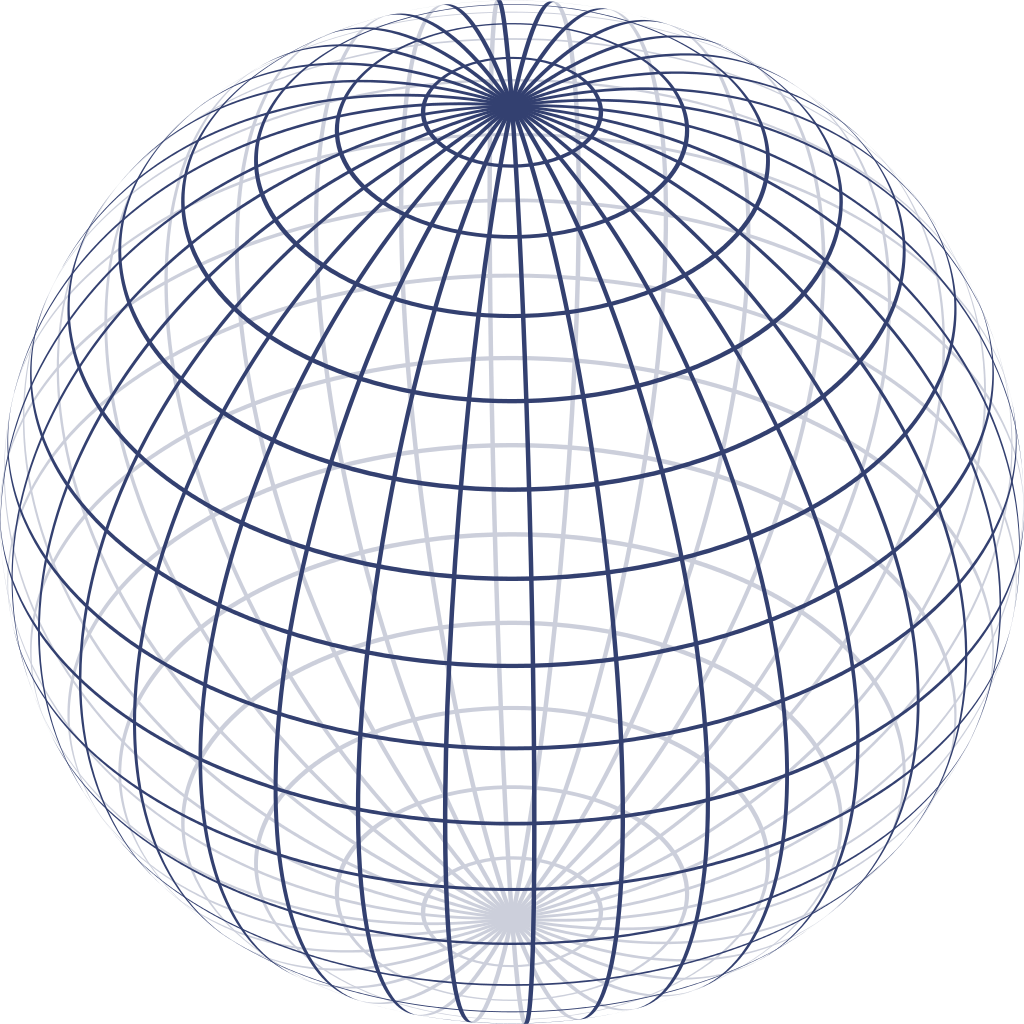
\includegraphics[width=3in]{./imagens/esfera}
\caption{Esfera $2$-dimensional}
\end{figure}

\subsection{O Espaço Projetivo}

\begin{defi}
Sejam $x,y \in \R^d$. A relação de \emph{equivalência homogênea} entre os pontos é definida por
	\begin{equation*}
	x : y \sse \exists t \in \R^* \qquad x = ty.
	\end{equation*}
\end{defi}

Essa relação é realmente uma relação de equivalência, pois tomando $t=1$ temos a reflexividade, tomando $\bar t = t\inv$ temos a simetria e tomando $t_1t_0$ temos a transitividade. A classe de equivalência de um ponto $x \in \R^d$ é a reta sem a origem de $\R^d$ que passa pela origem e por $x$, e é denotada por $[x_0 : \cdots : x_{d-1}] \coloneqq [x]$.

\begin{defi}
O \emph{espaço projetivo real} $d$-dimensional é o conjunto
	\begin{equation*}
	\pro\R^d \coloneqq \set{[x_0 : \cdots : x_d]}{x \in \R^{d+1}}.
	\end{equation*}
\end{defi}

Considerando os conjuntos
	\begin{equation*}
	A_i \coloneqq \set{[x_0 : \cdots : x_d] \in \pro\R^d}{x_i \neq 0}.
	\end{equation*}
e as funções
	\begin{align*}
	\func{\varphi_i}{A_i}{\R^d}{[x_0 : \cdots : x_d]}{\frac{1}{x_i}(x_0,\ldots,x_{i-1},x_{i+1},\ldots,x_d)},
	\end{align*}
cujas inversas são
	\begin{align*}
	\func{\varphi_i\inv}{\R^d}{A_i}{x}{[x_0:\ldots,x_{i-1}:1:x_i:,\ldots:x_{d-1}]}.
	\end{align*}

Uma descrição equivalente é
	\begin{equation*}
	\pro\R^d \coloneqq \set{\{x,-x\}}{x \in \S^d} = \S^d/\Z_2.
	\end{equation*}

\subsection{O Toro}

\begin{defi}
	O \emph{toro} $d$-dimensional é o conjunto
	\begin{equation*}
	\T^d \coloneqq \R^d / \Z^d.
	\end{equation*}
\end{defi}

\begin{figure}[!h]
\centering
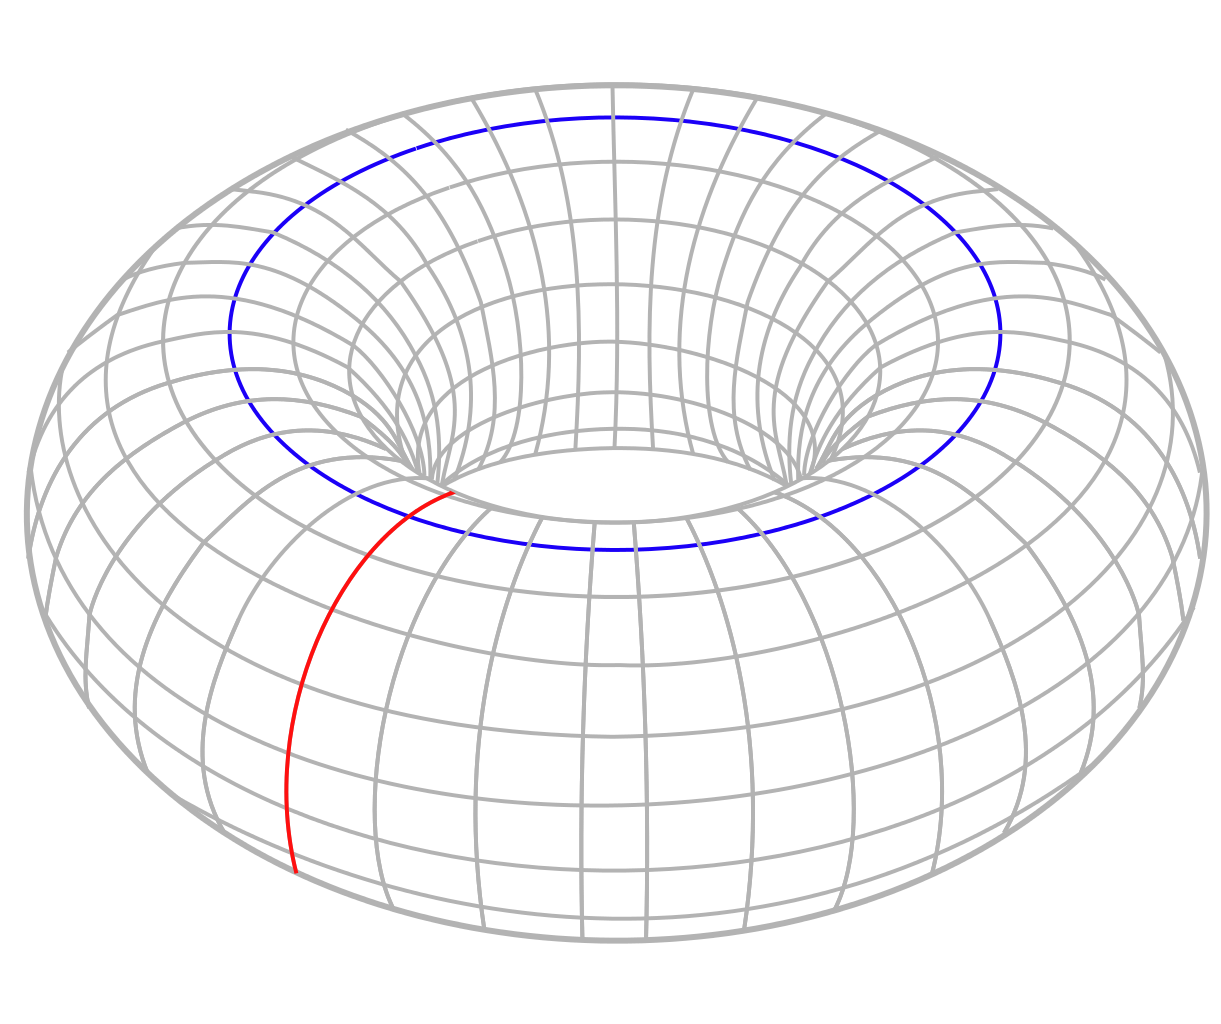
\includegraphics[width=3in]{./imagens/toro}
\caption{Toro}
\end{figure}

\subsection{Hiperboloide}

\begin{defi}
O \emph{hiperboloide} $d$-dimensional é o conjunto
	\begin{equation*}
	\Hip^d \coloneqq \set{(x,t) \in \R^d \times \R = \R^{d+1}}{\nor{x}^2+1=t^2 \e t>0}.
	\end{equation*}
\end{defi}


























